\chapter{Lambda Architecture}
\label{chap:lambda_architecture}

The Lambda architecture is a new solution for creating generic BigData systems \cite{MarzWarren201401}.
It provides model for scalable, fault-tolerant, distibuted processing of data.
It uses both batch and online processing to answer queries.
It provides human fault-tolerance, what is often overlooked in other approaches.
The Lambda architecture lets developer to concentrate on the logik and
algorithms, instead of thinking about maintainance of the system, e.g.
distributing computations, replication of dataset and how to manage intense grow of input data.

The core purpose of any information system is to answer specific queries having
data, gathered during functioning of the system.
Any query can be generically considered as a function of the whole dataset.
That means, that taking all available data, one can derive information, that
answers specific query.
[Running example]

Another important concept is that only raw data \mnote{raw data} must be
gathered in the system.
Its property is that it can not be derived from any other data.
It demands, nevertheless, that all types of queries, useful in the current
context, can be answered.
[Running example]

As a result of huge amounts of available data and its inherent rawness,
answering particular query is often unreasonably expensive or even infeasible. 
That is because query answer demands usually a piece of information, that is far
away from what raw data in the system describes.
It requires often execution of complex algorthims on the whole dataset.
In the BigData context that can mean hours of processing, while low-latency
response is typically a condition.
[Running example]

To solve this issue one can create batch views.
Batch view \mnote{batch view} is a specific data structure.
It contains derived data, that is a result of execution of specific algorithms
and aggregations on the whole dataset.
It is used for answering particular query.
Batch views are created in advance.
They can be used then in the query-time providing useful information.
[Running example]

Batch views are created in the infinite loop.
After the process of creation is completed, it starts again.
Processing all the data and creating batch views is high-latency operation.
It can take hours and even days to be done.
As a result batch views are always out-of-date.

To overcome this delay the Lambda architecture provides online processing.
It maintains additional data structures, called real-time views\mnote{real-time
view}.
They store information, derived from data arriving during current batch
processing.
Real-time views are normally different from batch views, and also more complex.
That is because they must be updated and available continuously, as new data
arrives.
This demands usage of such techniques like sketch algorithms.
It is described in all details in the particular chapter.
It worth to mention that real-time views contain often approximated information,
because of requirements they must obey.
But that is not a crucial problem, because they do not accumulate error for a
too long time.
Real-time view exists only during current batch processing.
When it is done, real-time views are dropped, and start to be created from the
beginning.

Summarizing, to answer the query system uses both things: batch views, computed
in the previous batch processing of the whole dataset, and real-time views,
gathering information from data coming during current batch processing.
Information from both types of views is then merged to provide answer to the
particular query.
Batch views provide information, that complete, but out-of-date for
several hours.
Real-time views contain information, gathered during current batch processing.

One more key aspect of the Lambda architecture, that makes a difference with
other approaches, is that human fault-tolerance is inherent.
Human fault-tolerance \mnote{human fault-tolerance} is robustness of the
system to mistakes in programming code.
This is important issue, because programmers' mistakes are guarantied.
As a result, deleting or updating the data in a wrong way is also possible.

The Lambda architecture doesn't allow to modify data. This is called
immutability\mnote{immutability}.
Data can be only added, and never deleted or updated.
This drammatically simplifies complexity of the system, because
maintainance of modifications in the distributed environment is not an easy
task.
But even more important, that mistakes in programming code can not ruin the
whole dataset anymore, what is a crucial requirement.
If the programming mistake occurs in the system, it can only write wrong data to
the dataset, that can be simply deleted later.
But all proper data is always safe. 

Immutability of data leads to completely different model of the way how
data is stored.
Instead of having simple tuple for a particular entity, every value of a tuple
is stored separately and has timestamp.
Such technique allows to have the whole history of editions of all attributes,
what can be useful to make queries, that use history of changes.
At the same time the actual value is the one with the oldest timestamp.

\authorsection{General structure}{VI}

Figure~\ref{fig:lambda_architecture} depicts general view of the Lambda
architecture.
In most common words, the system receives data from a particular source, and
answers the number of particular queries.
It consists itself of two main elements: batch part and real-time part.

Batch part in its turn comprises two parts: batch layer and serving layer.
Batch layer contains master dataset, that allows only appending data.
It executes computations on the whole master dataset to obtain batch views,
that are directly useful to answer queries.
Serving layer is the place where batch views reside.
It is also responsible for providing interface for making queries from those views.

Real-time part consists only of speed layer.  
Speed layer provides real-time views.
They contain sketches of data, that is being obesrved during ongoing batch
processing in the batch layer.
Speed layer is much more complex than batch layer, because of its incremental
nature.
And it provides only approximated results.
We discuss each layer in more details in particular chapters.

\begin{figure}[H]
  \centering
  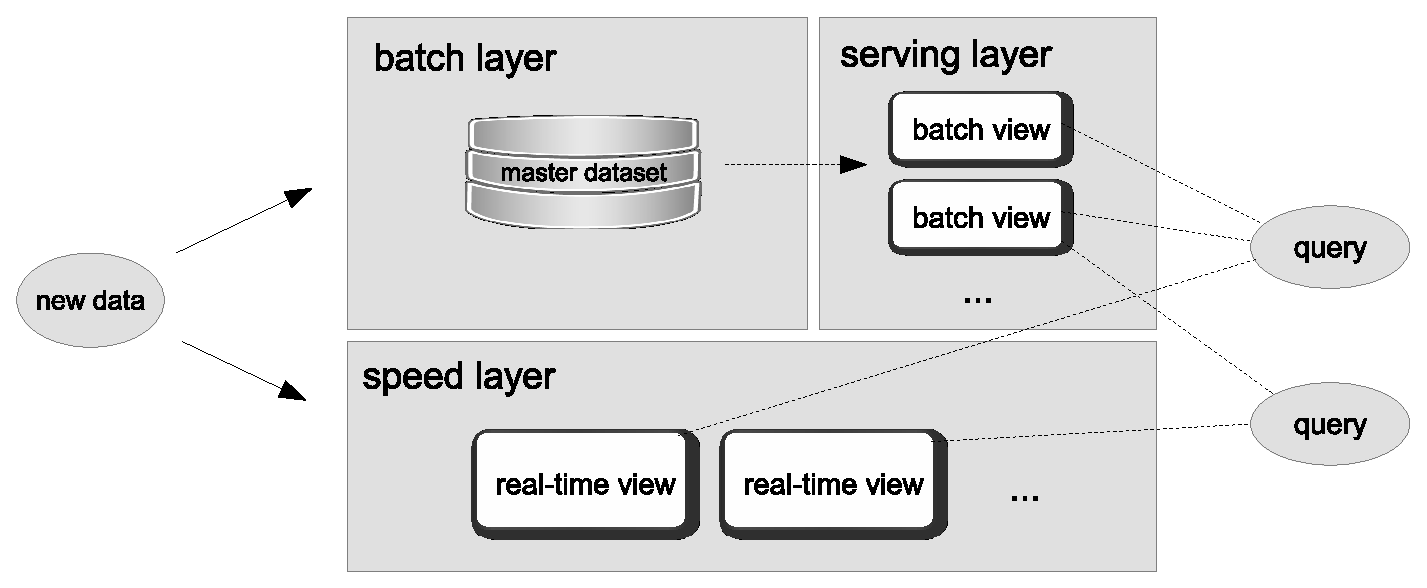
\includegraphics [width=0.9\textwidth]{images/LambdaArchitecture}
  \caption{General structure of the Lambda architecture}
  \label{fig:lambda_architecture}
\end{figure}

\authorsection{Batch layer}{VI}

Batch layer has two responsibilities: (i) it holds all data, that arrives from
the outer source, and (ii) it processes that data to compute batch views, useful
for answering queries.

Batch layer keeps data in master dataset.
\textit{Master dataset} \mnote{master dataset} is a main storage, that contains
all data, that ever came.
It is immutable, in the sense that it allows only addition of new records, and
does not allow modifications or deletions.
This property provides human foult-tolerance.
If master dataset is corrupted - all data is lost.
And data is of the most importance in our context.
Because of that master dataset must be carefully designed, set up and protected
from all types of failures, e.g software, hardware or human.

One can think about master dataset as of a very large list of records.
This is only a logical representation, however it is enough for current
discussion.
When new piece of data arrives into the system, it is added to the master
dataset.
As long as master dataset contains not only all data, but the whole history of
changes from the beginning of the deployment of the system, we can execute
queries on the whole history of those changes.

Data, stored in the master dataset, must be raw.
That means, that it can not be derived from any other data.
At the same time, it must be possible to answer all queries using it. 

Computation of batch views is being repeated continuously from scratch.
This is inherently distributed operation.
That means that developer does not have to think about concurrency and threads.
He only wrties simple one-threaded code, that is distributed then
automatically in the cluster.
MapReduce is a perfect example of a batch execution.
Apache Hadoop is an example of framework that can be used for computations in
the batch layer.

\authorsection{Serving layer}{VI}

Serving layer is a place where batch views are stored.
When batch layer computes batch views, it loads them into the serving layer.
Then serving layer indexes them for a fast access.
Serving layer is represented by a specific distibuted database. 
It can be swaped by new data, but it does not have ability to make random
writes.
That simplifies things extremely, because opportunity to make random writes
brings most of complexity in databases.
One example of database that can be used for serving layer is ElephantDB.

\authorsection{Speed layer}{VI}

The main purpose of the speed layer is the same as of batch part - to answer
queries.
As long as the batch layer computes views for several hours, speed layer is
dedicated to cover this interval, providing low-latency answers.
During the time of current batch processing, data coming to the system is stored
to master dataset as well as added incrementally to the real-time views in
speed layer.

This ability to update views on the fly makes speed layer much more complex.
It involves usage of databases, that allow random writes.
Algorithms, used to make online stream processing, are also usually more
complex.
Because of those issues, speed layer is more error prone, and takes more effort
from developer.
But real-time views are discarded every time, when batch layer completes
processing of batch views.
Such temporal nature of real-time views saves us from accumulation of
error.
This property of the Lambda architecture is called \textit{complexity isolation}\mnote{complexity isolation}.

\subsection{Computaition of real-time views}
To compute real-time views, one could consider the same approach as for batch
views, but use only new data for computations.
This would simulate batch processing on the much smaller scale.
Nevertheless, if we want to achieve latency of miliseconds, such approach is
not going to work.
Batch processing even on the scale of several gigabytes is not possible to do in
miliseconds.

To solve this issue we have to use completely different approach.
We do not consider the whole bunch of data, that has arrived during current
batch processing, for creating real-time views.
Instead, we incrementally update them with a small piece of data, everytime it
arrives.
This normally leads to only an approximated answers to the queries, provided by
real-time views.
But this is again not a problem, because error does not accumulate for too long.

\subsection{Storing real-time views}
Speed layer must obey low-latency requirement, and must allow to apply complex
incemental algorithms.
Having such demands, storing of real-time views requires much more properties
to be fulfilled:
1. Ability to make random reads. This is particularly important to make
answering queries fast.
2. Ability to make random writes. This is necessary, because we want to apply
incremental algorithms, that always demand this property.
3. Real-time view must be scalable, because amount of data to process can still
be of a huge size. That means, that distribtuion to many machines must be
possible.
4. Fault-tolerance is as usual an issue. Replication of real-time views is then
to accomplish.

Databases, that commonly obey these properties, are called \textit{NoSQL databases}\mnote{NoSQL databases}.
They store data using different data models.
One can choose specific database, that obeys his or her requirements to data
representation.
Sometimes batch and real-time views stores data in the same format.
But it is not always the case, because it is not always easy to execute the
same function in the batch and in the incremental way.
Also, as long as real-time views provide only temporal information, it is
usually possible to simplify data representation, becoming small approximation
error.
Because of those factors, it often happens, that your real-time views represent
data differently, than batch views.

\subsection{Issues of incremental computations}
Incremental computations are opposite to batch computations.
Batch computations imply, that we take the whole dataset, and compute
specific function on it.
This is usually easy to program, even though can take much time.

In case of incremental computations, we build specific data structure
continuously.
This data structure is called real-time view in our context.
It must be possible to update this data structure as well as to make requests
answering queries fast.
This two properies are the key to low-latency requirement satisfaction.

\subsection{Lifetime of data in it}
\subsection{Example Cassandra} 

